\begin{figure*}
  \centering
  % \begin{noindent}
  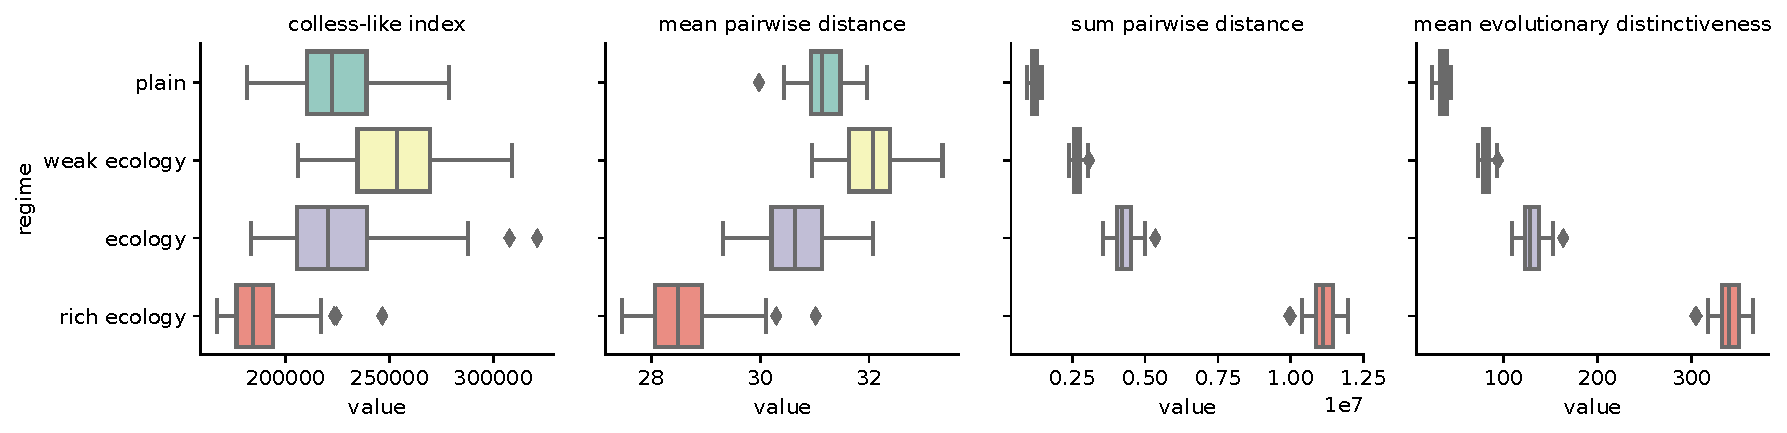
\includegraphics[width=\textwidth]{binder/binder/teeplots/col=phylometric+epoch=7+mut_distn=np.random.standard_normal+nuisance=spatial-structure+viz=boxplot+x=value+y=regime+ext=.pdf}
  % \end{noindent}
  \caption{%
    Distribution of phylometrics across the three surveyed ecological regimes and the control non-ecological regime---all with spatial population structure (i.e., island count 1,024).
    Phylometrics were calculated on perfect-fidelity simulation phylogenetic records.
    Results are for standard experimental conditions: gaussian mutation distribution at epoch 7 (generation 262,144).
    See Figure \ref{fig:perfect-tree-phylometrics-with-spatial-nuisance-sensitivity-analysis} for results under sensitivity analysis conditions.
    Sample sizes of $n=50$ replicates define each depicted distribution.
  }
  \label{fig:perfect-tree-phylometrics-with-spatial-nuisance}
\end{figure*}
